\section{Solution}

%----------------------------------------------------------------------------------------
%	PROJECT STRUCTURE SUBSECTION
%----------------------------------------------------------------------------------------
\subsection{Project Structure}
Project contains a header and source file for uart driver that was written in order to interact with peripheral which in our case is a virtual terminal.\\
\centerline{
	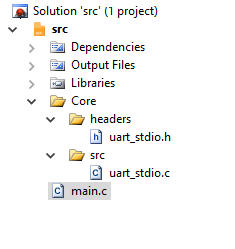
\includegraphics[width=0.6\textwidth]{solution/images/src.png}
}

%----------------------------------------------------------------------------------------
%	DEPENDENCES SUBSECTION
%----------------------------------------------------------------------------------------

\subsection{UART dependencies}
\begin{itemize}
	\item \textbf{\large stdio.h} - UART as a STD stream for IO Library
	\item \textbf{\large io.h} - MACRO definition for registers which makes our driver to work not only on ATMega32 but on more devices.
\end{itemize}

%----------------------------------------------------------------------------------------
%	DRIVER SUBSECTION
%----------------------------------------------------------------------------------------

\newpage
\subsection{UART Driver}
Procedures \&\& Functions: 
\begin{enumerate}
	\item \textbf{void uart\_stdio\_Init(void);} - initializing uart Baud frequency in order to make peripheral device to understand our signals correct.
    \item \textbf{void Int uart\_PutChar(char c, FILE *stream);} - printing on peripheral
\end{enumerate}

%----------------------------------------------------------------------------------------
%	MAIN PROGRAM SUBSECTION
%----------------------------------------------------------------------------------------

\subsection{Main program flow}
\begin{enumerate}
	\item Global variable declarations.
	\item UART Driver initialization
	\item Start infinite loop (Controller life cycle)
    \begin{enumerate}
		\item Increment counter variable
        \item Print counter to output(UART)
        \item Make a delay
	\end{enumerate}
\end{enumerate}

%----------------------------------------------------------------------------------------
%	PROTEUS SUBSECTION
%----------------------------------------------------------------------------------------

\newpage
\subsection{Circuit in Proteus}
I've connected MCU to Virtual Terminal. Because I use only data transmission on one direction (OUTPUT) we need to make sure that our MC Tx is connected to Peripheral Rx.\\\\
\centerline{
	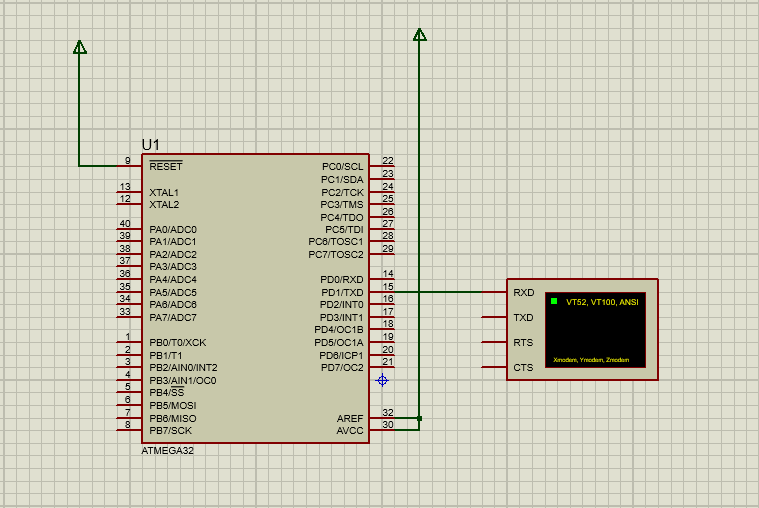
\includegraphics[width=1.0\textwidth]{solution/images/schematics.png}
}

%----------------------------------------------------------------------------------------
%	SIMULATION SUBSECTION
%----------------------------------------------------------------------------------------
\subsection{Simulation}
\centerline{
	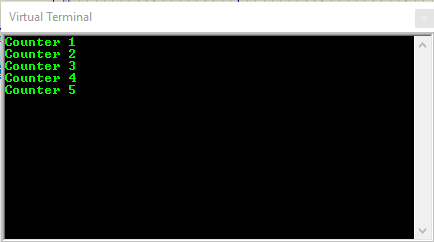
\includegraphics[width=1.0\textwidth]{solution/images/result.png}
}

